\subsection{Combining Parameter}

Thus far, we have not seen type B regions, that are not caused by overlapping type A regions.
We now want to change multiple parameters at the same time to imitate the function of the original model better.
For this, we introduce new parameters, $p_x$ and $p_y$, and define the actual model parameters dependent on those two.

\subsubsection{Defining $a_R = 1 + p_x$, $b_R = 2 \cdot px$, and $c_L = p_y$}

\todo{better imitation but nothing was found}

\subsubsection{Defining $a_R = 1 + 2 \cdot p_x$, $b_R = px$, and $c_L = p_y$}

This definition of $a_R$ and $b_R$ is similar to before, but now $p_x$ has double the effect on $a_R$ and half the effect on $b_R$.
It was created by accident since it does not imitate the original model as nicely as before.
\Cref{fig:quadratic.full.2aR1bR_cL.2d.full} shows the 2D scan of the different periods.
Regions we will have a closer look at, are marked with red rectangles.

\begin{figure}
    \centering
    \includegraphics[width=0.6\textwidth]{21_010_Quadratic_2aR1bR_cL/2D_Period_Selected/result.png}
    \caption{2D Scan of Periods of Quadratic Model with ...}
    \label{fig:quadratic.full.2aR1bR_cL.2d.full}
\end{figure}

The first enhanced region, shown in \Cref{fig:quadratic.full.2aR1bR_cL.2d.1}, has two areas with stable cycles of period 6 that overlap.
\Cref{fig:quadratic.regions.2aR1bR_cL.2d.1} shows the borders of the two regions.
It was created by halving the model and scanning for the borders of regions of different periods.
We will see that the bottom area is a type B area, and therefore the period in the halved model is double the period in the full model.

\begin{figure}
    \centering
    \begin{subfigure}{0.4\textwidth}
        \centering
        \includegraphics[width=\textwidth]{21_010_Quadratic_2aR1bR_cL/P6/2D_Period_P6/result.png}
        \caption{Periods}
        \label{fig:quadratic.full.2aR1bR_cL.2d.1}
    \end{subfigure}
    \begin{subfigure}{0.4\textwidth}
        \centering
        \includegraphics[width=\textwidth]{21_010_Quadratic_2aR1bR_cL/P6/2D_Regions_P6/result.png}
        \caption{Period Regions}
        \label{fig:quadratic.regions.2aR1bR_cL.2d.1}
    \end{subfigure}
    \caption{2D Scans of First Marked Region}
\end{figure}

\Cref{fig:quad.full.2aR1bR_cL.1.Cobwebs} shows cobweb diagrams at the three points marked in \Cref{fig:quadratic.full.2aR1bR_cL.2d.1,fig:quadratic.regions.2aR1bR_cL.2d.1}.
At point $A$, we have two stable coexisting cycles of period 6 with symbolic sequences $\A\B\C^3D$ and $\A^3\B\C\D$.
You can see them in \Cref{fig:quad.full.2aR1bR_cL.1.CobwebA}.
This region is therefore a type B region since we have two coexisting cycles that are symmetric by rotation.
At point $C$, we only have one stable cycle of period 6 with symbolic sequence $\A^2\B\C^3\D$.
\Cref{fig:quad.full.2aR1bR_cL.1.CobwebC} shows this cycle.
The upper region, therefore, is a type A region.
Both these regions overlap like in the original model.
\Cref{fig:quad.full.2aR1bR_cL.1.CobwebB} shows the stable cycles at point $C$ in the overlapping area.
\todo{similarity to overlap in og model}

\begin{figure}
    \centering
    \begin{subfigure}{0.3\textwidth}
        \centering
        \includegraphics[width=\textwidth]{21_010_Quadratic_2aR1bR_cL/P6/Cobweb_P6_A/result.png}
        \caption{At Point A}
        \label{fig:quad.full.2aR1bR_cL.1.CobwebA}
    \end{subfigure}
    \begin{subfigure}{0.3\textwidth}
        \centering
        \includegraphics[width=\textwidth]{21_010_Quadratic_2aR1bR_cL/P6/Cobweb_P6_B/result.png}
        \caption{At Point B}
        \label{fig:quad.full.2aR1bR_cL.1.CobwebB}
    \end{subfigure}
    \begin{subfigure}{0.3\textwidth}
        \centering
        \includegraphics[width=\textwidth]{21_010_Quadratic_2aR1bR_cL/P6/Cobweb_P6_C/result.png}
        \caption{At Point C}
        \label{fig:quad.full.2aR1bR_cL.1.CobwebC}
    \end{subfigure}
    \caption{Cobwebs at Different Points}
    \label{fig:quad.full.2aR1bR_cL.1.Cobwebs}
\end{figure}

The second, lower, enhanced region has two areas with stable cycles of period 8 that overlap.
\Cref{fig:quadratic.full.2aR1bR_cL.2d.2} shows that region, while \Cref{fig:quadratic.regions.2aR1bR_cL.2d.2} shows the borders of the two areas, like before.

\begin{figure}
    \centering
    \begin{subfigure}{0.4\textwidth}
        \centering
        \includegraphics[width=\textwidth]{21_010_Quadratic_2aR1bR_cL/P8/2D_Period_P8/result.png}
        \caption{Periods}
        \label{fig:quadratic.full.2aR1bR_cL.2d.2}
    \end{subfigure}
    \begin{subfigure}{0.4\textwidth}
        \centering
        \includegraphics[width=\textwidth]{21_010_Quadratic_2aR1bR_cL/P8/2D_Regions_P8/result.png}
        \caption{Period Regions}
        \label{fig:quadratic.regions.2aR1bR_cL.2d.2}
    \end{subfigure}
    \caption{2D Scans of Second Marked Region}
\end{figure}

\Cref{fig:quad.full.2aR1bR_cL.2.Cobwebs} shows cobweb diagrams at the three points marked in \Cref{fig:quadratic.full.2aR1bR_cL.2d.2,fig:quadratic.regions.2aR1bR_cL.2d.2}.
We can see that the lower area is again of type B, we have two coexisting stable cycles of period 8 with symbolic sequences $\A^2\B\C^4\D$ and $\A^4\B\C^2\D$.
\Cref{fig:quad.full.2aR1bR_cL.2.CobwebA} shows these cycles at the point $A$.
As before, the other area is of type B and has one stable cycle of period 8 with the symbolic sequence $\A^3\B\C^3\D$.
You can see it in \Cref{fig:quad.full.2aR1bR_cL.2.CobwebC}, it was generated at the point $C$.

\begin{figure}
    \centering
    \begin{subfigure}{0.3\textwidth}
        \centering
        \includegraphics[width=\textwidth]{21_010_Quadratic_2aR1bR_cL/P8/Cobweb_P8_A/result.png}
        \caption{At Point A}
        \label{fig:quad.full.2aR1bR_cL.2.CobwebA}
    \end{subfigure}
    \begin{subfigure}{0.3\textwidth}
        \centering
        \includegraphics[width=\textwidth]{21_010_Quadratic_2aR1bR_cL/P8/Cobweb_P8_B/result.png}
        \caption{At Point B}
        \label{fig:quad.full.2aR1bR_cL.2.CobwebB}
    \end{subfigure}
    \begin{subfigure}{0.3\textwidth}
        \centering
        \includegraphics[width=\textwidth]{21_010_Quadratic_2aR1bR_cL/P8/Cobweb_P8_C/result.png}
        \caption{At Point C}
        \label{fig:quad.full.2aR1bR_cL.2.CobwebC}
    \end{subfigure}
    \caption{Cobwebs at Different Points}
    \label{fig:quad.full.2aR1bR_cL.2.Cobwebs}
\end{figure}
